\subsection{Curvas En Variedades}\label{Subsección: Curvas En Variedades}
Una de las ideas que podemos trasladar del cálculo ordinario al cálculo que estamos realizando en variedades suaves es la idea de curva definida en una superficie y la velocidad de la misma, nombre que viene inspirado de la utilidad en la física que estos conceptos tiene, ya que podemos pensar en la curva como una trayectoria y su derivada como su velocidad.
En nuestro caso al estar trabajando con variedades estas serán nuestras \enquote{superficies} y, si bien no podemos simplemente derivar, sí podemos asociar a cada punto de la curva un vector en el espacio tangente.

\begin{definition}[Curva en una Variedad]
  \label{Definición: Curva en Variedades}
	Sea $M$ una variedad y sea $\gamma: I \subset \R \to M$ un mapa continuo, donde $I$ es un intervalo, diremos que $\gamma$ es una \it{curva sobre $M$}. Además, si el mapa $\gamma: I \subset \R \to M$ es suave diremos que $\gamma$ es una curva suave.
\end{definition}

Notemos que para la definición de curva solo estamos pidiendo continuidad, no suavidad. Una curva puede estar definida en una variedad topológica para la cual no es posible dar una estructura suave. Sin embargo, para poder definir la velocidad es necesario que el espacio tangente esté definido, por lo que pediremos que tanto las variedades como las curvas sean suaves.

\begin{figure}[h]
  \centering
  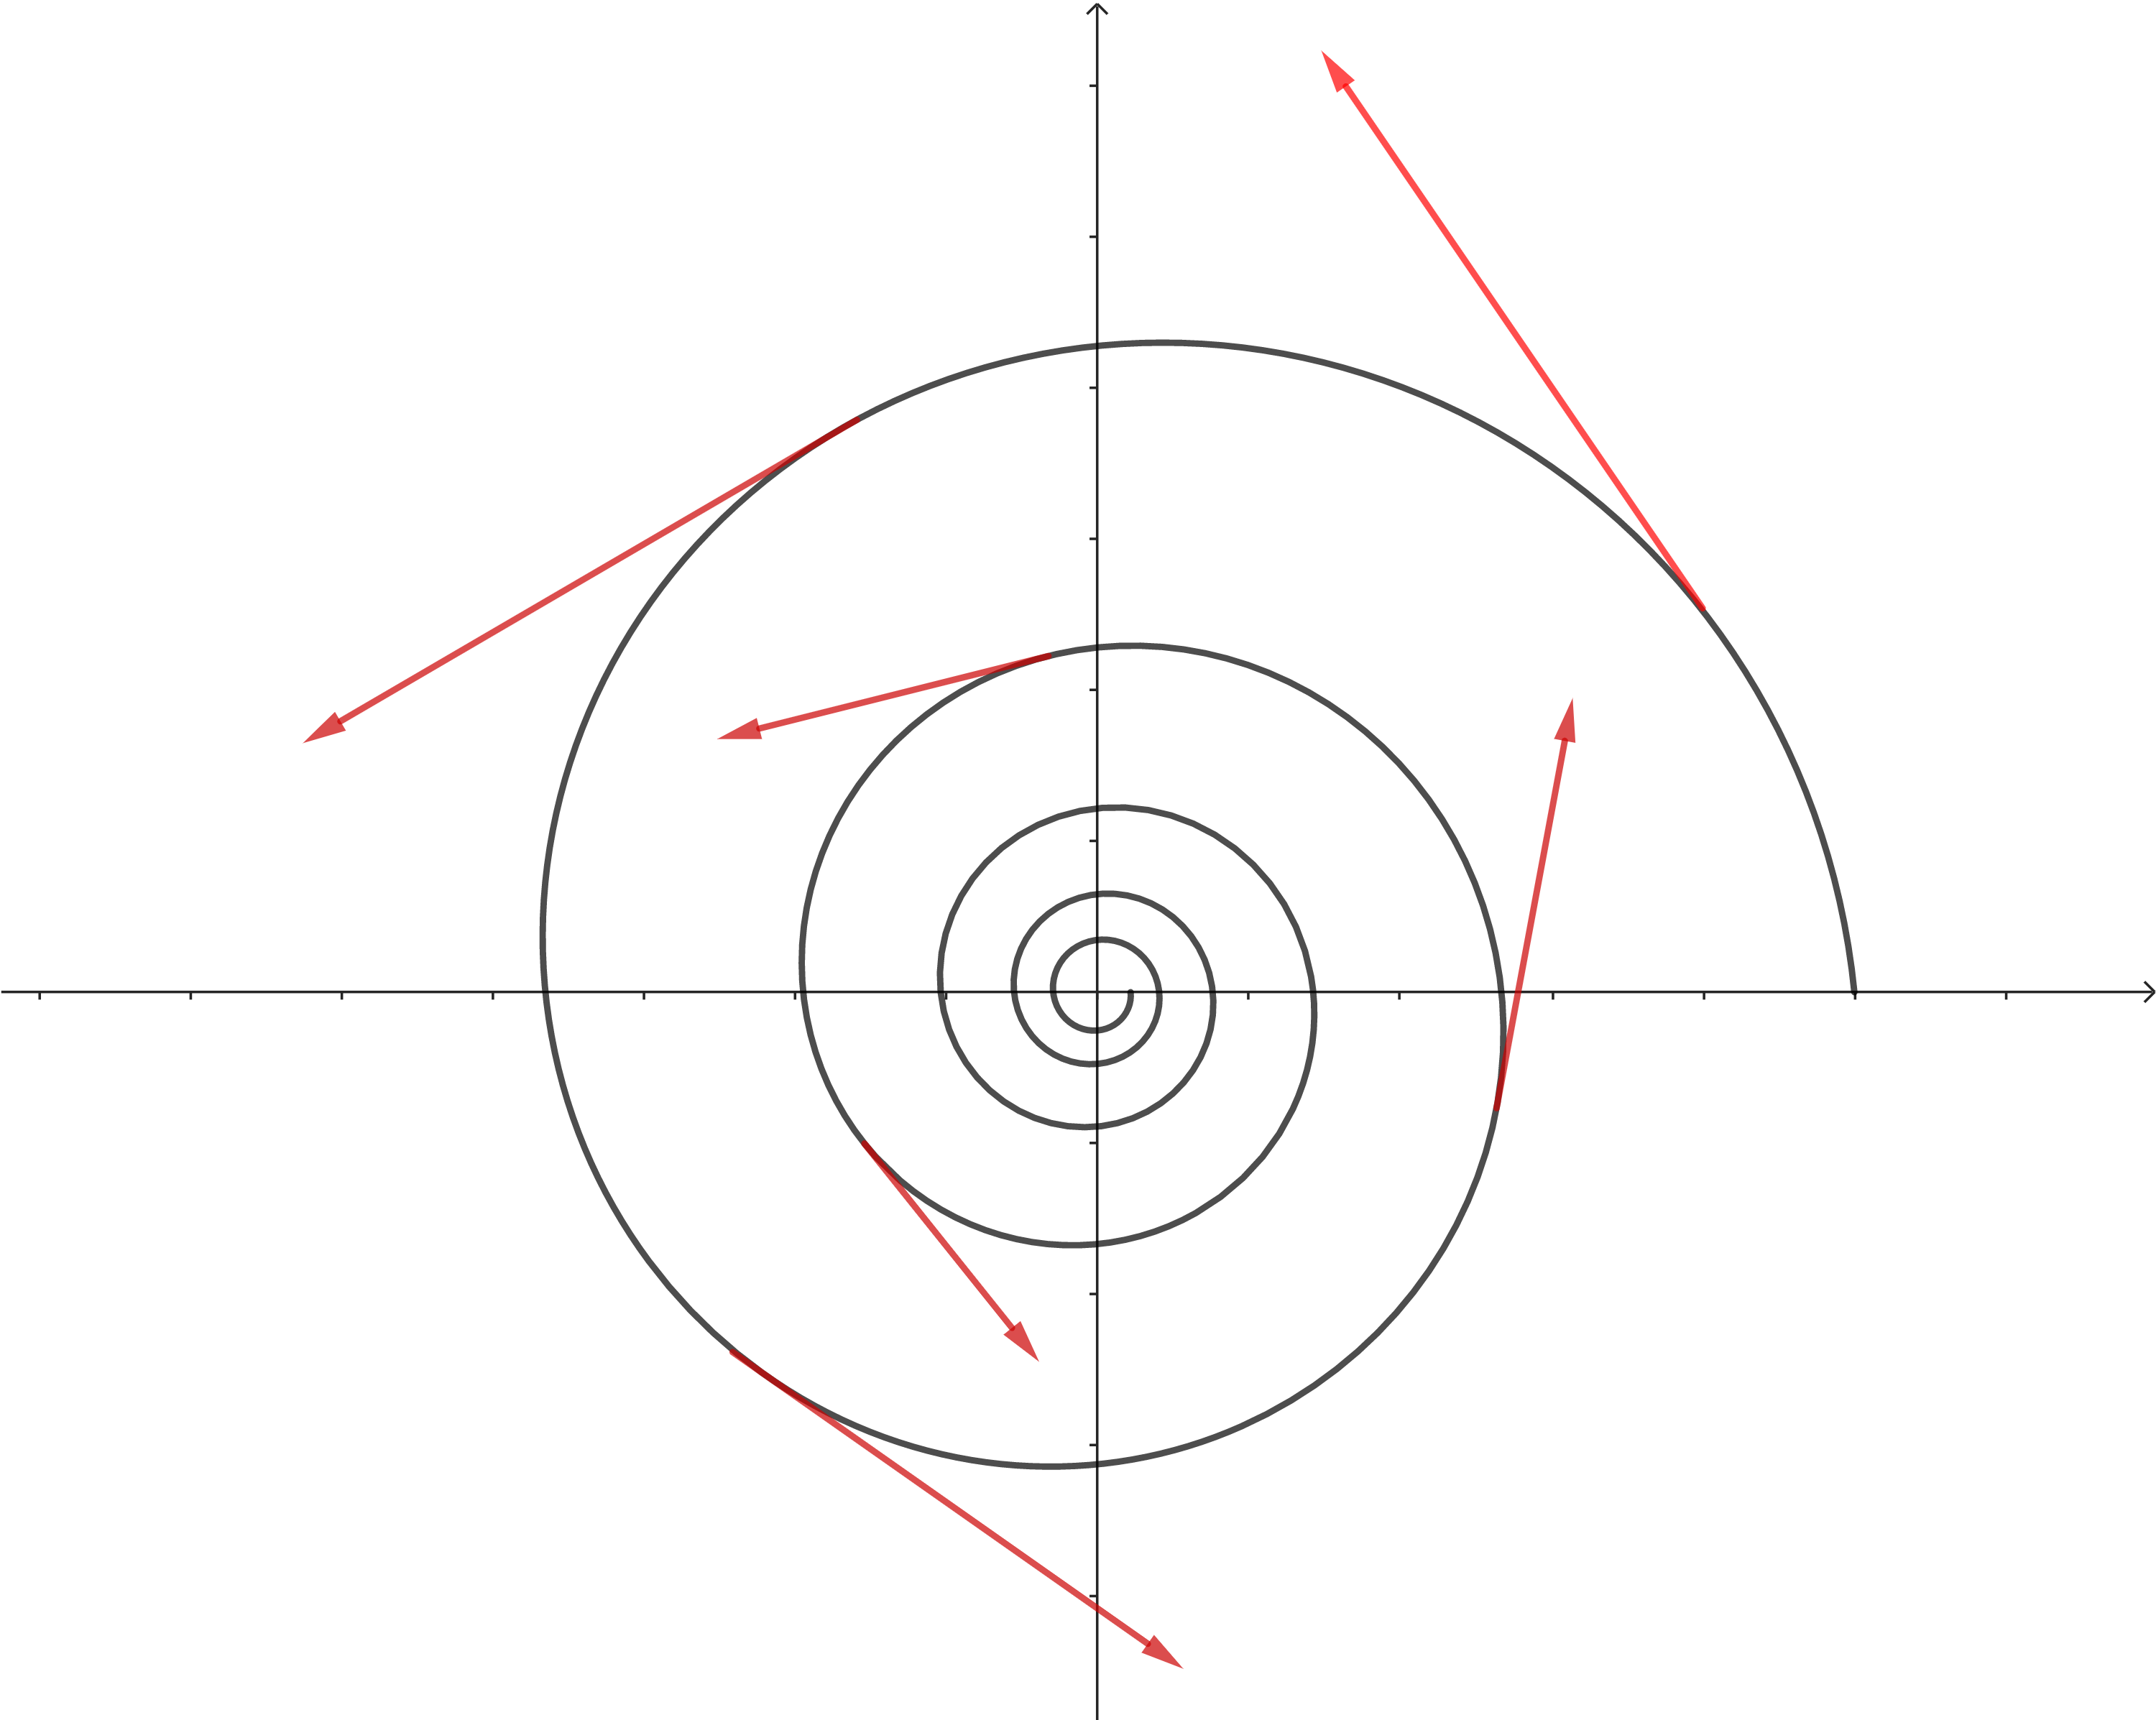
\includegraphics[width=0.5\textwidth]{~/Tesis/Figuras/A-Figuras/CurvaLogaritmica.png}
  \caption{Figura}
\end{figure}


\begin{definition}[Velocidad de una Curva]
	Sea $M$ una variedad suave, $\gamma: I \to M$ una curva suave y $t_0 \in I$. Definimos la \it{velocidad de $\gamma$ en $t_0$}, la cual denotaremos como $\gamma'(t_0)$, como el vector:
	\[
		\gamma'(t_0)
		=
		d\gamma\left( \left.  \frac{d}{dt}\right|_{t_0} \right)
		\in
		T_{\gamma(t_0)}(M).
	\]
	Donde $\frac{d}{dt}$ es la base estándar en $T\R$.
\end{definition}

Al estar definida como un vector en el espacio tangente actuará sobre funciones suaves de $M$ del siguiente modo: Dada una función suave $f: M \to \R$, la regla de la cadena nos dice que:
\begin{align*}
	\gamma'(t_0) f & =d\gamma\left(\left.\frac{d}{dt}\right|_{t_0} \right)f \\
	               & = \left. \frac{d}{dt} \right|_{t_0} (f \circ \gamma)   \\
	               & = (f \circ \gamma)' (t_0).
\end{align*}

Esta última igualdad nos dice que esta es una derivada en el sentido usual, dado que $\gamma: \R \to M$ y $f: M \to \R$ por lo que $f \circ \gamma: \R \to \R$. Si consideramos a la variedad $M=\R^n$ o algún subconjunto abierto de $\R^n$ esta definición coincide con la definición dada por do \textcite{do2016differential}.

Si tomamos una carta suave $(U,\phi) = (U,\phi_1,\dots,\phi_n)$ en una variedad suave $M$ y dicha carta contiene a un punto $\gamma(t_0)$, donde $\gamma$ es una curva en $M$, podemos dar la representación coordenada de $\gamma$, en una vecindad suficientemente pequeña de $t_0$ como $\gamma(t) = (\gamma_1(t), \dots, \gamma_n(t))$, y por la fórmula que tenemos para representar al diferencial en coordenadas tendremos que gamma se puede escribir como:
\[
	\gamma'(t_0)=\sum_{i=1}^{n}\frac{d \gamma_i}{dt} (t_0)
	\left. \frac{\partial}{\partial \phi_i} \right|_{\gamma(t_0)}.
\]

\begin{example}
	Consideremos la función $\gamma: (0,\pi) \to \S^{1}$ definida por
	\[
		\gamma(t) = (\cos (t), \sin (t)).
	\]

	Esta función es suave en ambas componentes, en particular es continua, por lo que será una curva en $\S^1$ y por ser suave podremos hablar de su velocidad en cada punto $t_0 \in (0,\pi)$.

	La base en coordenadas polares para el espacio tangente de $\S^{1}$ puede ser dada como $\left( \frac{\partial}{\partial r} , \frac{\partial}{\partial \theta} \right)$. Si quisiéramos dar la velocidad de la curva en un punto, digamos $t_0 = \frac{\pi}{4}$, dicha curva tendrá su representación en coordenadas del siguiente modo:

	\begin{align*}
		\gamma'(t_0) & = \frac{d \gamma_1}{dt}\left( \frac{\pi}{4} \right)
		\left.\frac{\partial}{\partial r} \right|_{\gamma(\frac{\pi}{4})} +
		\frac{d \gamma_2}{dt} \left(\frac{\pi}{4} \right)
		\left.\frac{\partial}{\partial\theta} \right|_{\gamma(\frac{\pi}{4})} \\
		             & = -\sin \left(\frac{\pi}{4}\right)
		\left. \frac{\partial}{\partial r} \right|_{\gamma(\frac{\pi}{4})} +
		\cos \left( \frac{\pi}{4} \right)
		\left.\frac{\partial}{\partial\theta}\right|_{\gamma(\frac{\pi}{4})}  \\
		             & = -\frac{\sqrt{2}}{2}
		\left. \frac{\partial}{\partial r} \right|_{\gamma(\frac{\pi}{4})}
		+ \frac{\sqrt{2}}{2}
		\left. \frac{\partial}{\partial\theta} \right|_{\gamma(\frac{\pi}{4})}.
	\end{align*}
\end{example}

\begin{theorem}
	Supongamos que $M$ es una variedad suave y que $p \in M$. Cada vector $\omega \in T_p(M)$ es la velocidad de alguna curva suave en $M$.
\end{theorem}

\begin{proof}
	Tomemos algún punto $p \in M$, y sea $(U,\phi) = (U,\phi_1, \dots, \phi_n)$ una carta suave en $M$ centrada en $p$. Tomemos cualquier vector $\omega \in T_p(M)$, este vector puede ser expresado en como una combinación lineal en términos de la base coordenada de $T_p(M)$ del siguiente modo:
	\[
		\omega = \sum_{i=1}^{n} v_i \left.\frac{\partial}{\partial \phi_i}\right|_{p}.
	\]

	donde $v_i$ son constantes que dependen de $\omega$. Para un $\epsilon > 0$ suficientemente pequeño podemos considerar la curva $\gamma: (-\epsilon, \epsilon) \to U$ cuya representación coordenada sea:
	\[
		\gamma(t) = \phi^{-1}(tv_1, \dots, tv_n), \quad t \in (-\epsilon,\epsilon).
	\]

	Esta será una curva suave en $M$, y utilizando la representación en coordenadas dada anteriormente para la velocidad tendremos:
	\begin{align*}
		\gamma'(0) & = \sum_{i=1}^{n} \frac{d\gamma_i}{dt}(0)
		\left.  \frac{\partial}{\partial \phi_i}\right|_{\gamma(0)}                         \\
		           & = \sum_{i=1}^{n} \frac{d (tv_i)}{dt}(0)
		\left. \frac{\partial}{\partial \phi_i} \right|_{\gamma(0)= p}                      \\
		           & = \sum_{i=1}^{n} v_i \left. \frac{\partial}{\partial \phi_i} \right|_p \\
		           & = \omega.
	\end{align*}
\end{proof}

Conocer la velocidad de una curva es muy útil no solamente por su posible interpretación física, también nos da una manera alternativa para poder calcular el diferencial de un mapa, que es especialmente útil cuando tenemos un mapa que no está representado en coordenadas estándar de forma explícita, como se verá con los siguientes dos resultados.

\begin{lemma}
	Sean $M$ y $N$ variedades suaves, $F: M \to N$ un mapa suave, y sea $\gamma: I \to M$ una curva suave. Para cada $t_0 \in I$ la velocidad de la curva compuesta en $t=t_0$ está dada por:
	\[ (F \circ \gamma)'(t_0) = dF(\gamma'(t_0)). \]
\end{lemma}

\begin{proof}
	Bastará aplicar la definición de velocidad de una curva y el corolario \ref{Corolario: Propiedades de los diferenciales}, de tal manera que se obtendrá la siguiente cadena de igualdades:
	\begin{align*}
		(F \circ \gamma)'(t_0) & = d(F \circ \gamma)'
		\left(\left. \frac{d}{dt}\right|_{t_0} \right)                                              \\
		                       & = dF \circ d \gamma \left( \left. \frac{d}{dt}\right|_{t_0}\right) \\
		                       & = dF(\gamma'(t_0)).
	\end{align*}
\end{proof}

\begin{corollary}
	Sean $M$ y $N$ variedades suaves, $F: M \to N$ un mapa suave, $p \in M$ y $\omega \in T_p(M)$. Entonces para cualquier curva suave $\gamma: I \to M$ tal que $0 \in I$, $\gamma(0) = p$ y $\gamma'(0) = \omega$ se tendrá:
	\[
		d_pF(\omega) = (F \circ \gamma)'(0).
	\]
\end{corollary}
